%% ----------------------------------------------------------------
%% Report.tex
%% ---------------------------------------------------------------- 
\documentclass{ecsreport}      % Use the Report Style
\graphicspath{{../Figures/}}   % Location of your graphics files
\usepackage{natbib}            % Use Natbib style for the refs.
\usepackage{longtable}         % Use long table to span tables across pages
\hypersetup{colorlinks=false}   % Set to false for black/white printing
\let\cleardoublepage\clearpage
%% ----------------------------------------------------------------
%% Definitions.tex
%% ---------------------------------------------------------------- 
\newcommand{\BibTeX}{{\rm B\kern-.05em{\sc i\kern-.025em b}\kern-.08em T\kern-.1667em\lower.7ex\hbox{E}\kern-.125emX}}

%% People
\newcounter{address}
\setcounter{address}{1}
\renewcommand{\theaddress}{\textsuperscript{\fnsymbol{address}}}
\newcommand{\address}[1]{\refstepcounter{address}\theaddress#1\\}
\newcommand{\Name}[3]{\texorpdfstring{\href{mailto:#3}{#2}#1}{#2}\xspace}
\newcommand{\SteveRGunn}[1]{\Name{#1}{Steve R. Gunn}{S.R.Gunn@ecs.soton.ac.uk}}

%% Dingbats
\newcommand{\tick}{\ding{51}}
\newcommand{\cross}{\ding{55}}

%% Calculus
\newcommand{\pd}[2]{\ensuremath{\frac{\partial #1}{\partial #2}}\xspace}
\newcommand{\fd}[2]{\ensuremath{\frac{d #1}{d #2}}\xspace}
\newcommand{\dint}{\ensuremath{\int\!\!\!\int}\xspace}
\newcommand{\tint}{\ensuremath{\int\!\!\!\int\!\!\!\int}\xspace}

%% Math Sets
\newcommand{\Q}[1]{\ensuremath{\mathbb{#1}}\xspace}
\newcommand{\R}{\Q{R}}

%% Matrix, Vector
\newcommand{\V}[1]{\ensuremath{\boldsymbol{#1}}\xspace}
\newcommand{\M}[1]{\ensuremath{\boldsymbol{#1}}\xspace}
\newcommand{\0}{\V{0}}
\newcommand{\1}{\V{1}}
\newcommand{\I}{\M{I}}

%% Math Functions
\newcommand{\F}[1]{\ensuremath{\mathrm{#1}}\xspace}
\newcommand{\sgn}{\F{sgn}}
\newcommand{\tr}{\F{trace}}
\newcommand{\diag}{\F{diag}}

%% Math Names
\newcommand{\N}[1]{\ensuremath{\mathit{#1}}\xspace}

%% Data
\newcommand{\mc}[1]{\ensuremath{\mathcal{#1}}\xspace}
\newcommand{\Hyp}{\mc{H}}
\newcommand{\D}{\mc{D}}

%% Kernel
\newcommand{\K}{\M{K}}
\newcommand{\eins}{\texorpdfstring{\ensuremath{\epsilon}}{\textepsilon}-insensitive\xspace}
\newcommand{\e}{\ensuremath{\epsilon}\xspace}
\newcommand{\Bxi}{\ensuremath{\boldsymbol{\xi}}\xspace}
\newcommand{\Kanova}{\ensuremath{\mathit{K_{ANOVA}}}\xspace}
\newcommand{\Kspline}{\ensuremath{\mathit{K_{spline}}}\xspace}

%% Bayesian
\newcommand{\MP}{\ensuremath{\mathit{{\scriptscriptstyle \hspace{-1.5pt}M\hspace{-1.5pt}P}}}\xspace}
\newcommand{\ML}{\ensuremath{\mathit{{\scriptscriptstyle \hspace{-1.5pt}M\hspace{-1.5pt}L}}}\xspace}
\newcommand{\Qw}{\ensuremath{Q_{\w}(\w)}\xspace}
\newcommand{\Qa}{\ensuremath{Q_{\Ba}(\Ba)}\xspace}
\newcommand{\Qb}{\ensuremath{Q_{\beta}(\beta)}\xspace}
\newcommand{\wMPab}{\ensuremath{\w_{\MP|\bar {\Ba},\bar \beta}}\xspace}
\newcommand{\wMP}{\ensuremath{\w_{\MP}}\xspace}
\newcommand{\yMP}{\ensuremath{y_{\MP}}\xspace}
\newcommand{\BaMP}{\ensuremath{\Ba_{\hspace{1pt}\MP}}\xspace}
\newcommand{\aMP}{\ensuremath{\alpha_{\hspace{1pt}\MP}}\xspace}
\newcommand{\bMP}{\ensuremath{\beta_{\hspace{1pt}\MP}}\xspace}
\newcommand{\Sab}{\ensuremath{\M{\Sigma}_{\bar \Ba,\bar \beta}}\xspace}
\newcommand{\Ba}{\ensuremath{\boldsymbol{\alpha}}\xspace}
\newcommand{\Bb}{\ensuremath{\boldsymbol{\beta}}\xspace}
\newcommand{\Bm}{\ensuremath{\boldsymbol{\mu}}\xspace}
\newcommand{\BL}{\ensuremath{\boldsymbol{\Lambda}}\xspace}
\newcommand{\BPhi}{\ensuremath{\boldsymbol{\Phi}}\xspace}
\newcommand{\SMP}{\ensuremath{\M{\Sigma}_{\MP}}\xspace}

\newcommand{\Pa}{\ensuremath{P(\alpha|\mathcal{H})}\xspace}
\newcommand{\Pb}{\ensuremath{P(\beta|\mathcal{H})}\xspace}
\newcommand{\Pab}{\ensuremath{P(\alpha,\beta|\mathcal{H})}\xspace}
\newcommand{\Pw}{\ensuremath{P(\w|\mathcal{H})}\xspace}
\newcommand{\PD}{\ensuremath{P(\D|\mathcal{H})}\xspace}
\newcommand{\PwIa}{\ensuremath{P(\w|\alpha,\mathcal{H})}\xspace}
\newcommand{\PDIwb}{\ensuremath{P(\D|\w,\beta,\mathcal{H})}\xspace}
\newcommand{\PDwab}{\ensuremath{P(\D,\w,\alpha,\beta|\mathcal{H})}\xspace}
\newcommand{\PDIw}{\ensuremath{P(\D|\w,\mathcal{H})}\xspace}
\newcommand{\PwID}{\ensuremath{P(\w|\D,\mathcal{H})}\xspace}
\newcommand{\PwabID}{\ensuremath{P(\w,\alpha,\beta|\D,\mathcal{H})}\xspace}

\newcommand{\PanH}{\ensuremath{P(\alpha)}\xspace}
\newcommand{\PbnH}{\ensuremath{P(\beta)}\xspace}
\newcommand{\PabnH}{\ensuremath{P(\alpha,\beta)}\xspace}
\newcommand{\PwnH}{\ensuremath{P(\w)}\xspace}
\newcommand{\PDnH}{\ensuremath{P(\D)}\xspace}
\newcommand{\PwIanH}{\ensuremath{P(\w|\alpha)}\xspace}
\newcommand{\PDIwbnH}{\ensuremath{P(\D|\w,\beta)}\xspace}
\newcommand{\PDwabnH}{\ensuremath{P(\D,\w,\Ba,\beta)}\xspace}
\newcommand{\PDIwnH}{\ensuremath{P(\D|\w)}\xspace}
\newcommand{\PwIDnH}{\ensuremath{P(\w|\D)}\xspace}
\newcommand{\PwabIDnH}{\ensuremath{P(\w,\alpha,\beta|\D)}\xspace}

\newcommand{\PDwBab}{\ensuremath{P(\D,\w,\Ba,\beta|\mathcal{H})}\xspace}
\newcommand{\PwIBa}{\ensuremath{P(\w|\Ba,\mathcal{H})}\xspace}
\newcommand{\PBab}{\ensuremath{P(\Ba,\beta|\mathcal{H})}\xspace}
\newcommand{\PwBabID}{\ensuremath{P(\w,\Ba,\beta|\D,\mathcal{H})}\xspace}

\newcommand{\PBanH}{\ensuremath{P(\Ba)}\xspace}
\newcommand{\PwIBanH}{\ensuremath{P(\w|\Ba)}\xspace}

%% Snakes
\newcommand{\Esnake}{\ensuremath{\mathit{E_{snake}}}\xspace}
\newcommand{\Eimage}{\ensuremath{\mathit{E_{image}}}\xspace}
\newcommand{\Econt}{\ensuremath{\mathit{E_{cont}}}\xspace}
\newcommand{\Ecurv}{\ensuremath{\mathit{E_{curv}}}\xspace}
\newcommand{\Eint}{\ensuremath{\mathit{E_{int}}}\xspace}
\newcommand{\Eext}{\ensuremath{\mathit{E_{ext}}}\xspace}
\newcommand{\Eterm}{\ensuremath{\mathit{E_{term}}}\xspace}
\newcommand{\Eline}{\ensuremath{\mathit{E_{line}}}\xspace}
\newcommand{\Eedge}{\ensuremath{\mathit{E_{edge}}}\xspace}
\newcommand{\Econ}{\ensuremath{\mathit{E_{con}}}\xspace}
\newcommand{\Eangle}{\ensuremath{\mathit{E_{angle}}}\xspace}
\newcommand{\Elshape}{\ensuremath{\mathit{E_{lshape}}}\xspace}
\newcommand{\Eedgedir}{\ensuremath{\mathit{E_{edgedir}}}\xspace}
\newcommand{\Emodel}{\ensuremath{\mathit{E_{model}}}\xspace}
\newcommand{\wte}{\ensuremath{\mathit{w_{term}}}\xspace}
\newcommand{\wli}{\ensuremath{\mathit{w_{line}}}\xspace}
\newcommand{\wed}{\ensuremath{\mathit{w_{edge}}}\xspace}
\newcommand{\wco}{\ensuremath{\mathit{w_{con}}}\xspace}

%% Environments
\newcounter{alg}
\newenvironment{algorithm}[1]
{
    \stepcounter{alg}
    \begin{table}[htb]
    \centering
    \begin{tabular}[t]{ll}
    \hline&\\
    \multicolumn{2}{l}{\bf Algorithm \arabic{alg}: #1}\\&\\
} {
    &\\
    \hline
    \end{tabular}
    \end{table}
}
            % Include your abbreviations
\usepackage{dirtytalk}
\usepackage[utf8]{inputenc}
\usepackage{siunitx}
\usepackage{graphicx}
\usepackage{listings}
\usepackage{color}
\usepackage{appendix}
%\usepackage{minted}
\usepackage{color}
%\usepackage{gensymb}
\usepackage{dirtytalk}
\usepackage{float}

\usepackage{pdfpages}

\definecolor{dkgreen}{rgb}{0,0.6,0}
\definecolor{gray}{rgb}{0.5,0.5,0.5}
\definecolor{mauve}{rgb}{0.58,0,0.82}
\definecolor{lightgray}{rgb}{.9,.9,.9}
\definecolor{darkgray}{rgb}{.4,.4,.4}
\definecolor{purple}{rgb}{0.65, 0.12, 0.82}

\lstset{frame=tb,
  aboveskip=3mm,
  belowskip=3mm,
  showstringspaces=false,
  columns=flexible,
  basicstyle={\small\ttfamily},
  numberstyle=\tiny\color{gray},
  keywordstyle=\color{blue},
  commentstyle=\color{dkgreen},
  stringstyle=\color{mauve},
  breaklines=true,
  breakatwhitespace=true,
  tabsize=3,
  numbers=left
}

\lstdefinelanguage{JavaScript}{
  keywords={break, case, catch, continue, debugger, default, delete, do, else, false, finally, for, function, if, in, instanceof, new, null, return, switch, this, throw, true, try, typeof, var, void, while, with},
  morecomment=[l]{//},
  morecomment=[s]{/*}{*/},
  morestring=[b]',
  morestring=[b]",
  ndkeywords={class, export, boolean, throw, implements, import, this},
  keywordstyle=\color{blue}\bfseries,
  ndkeywordstyle=\color{darkgray}\bfseries,
  identifierstyle=\color{black},
  commentstyle=\color{purple}\ttfamily,
  stringstyle=\color{red}\ttfamily,
  sensitive=true
}

\newcommand\invisiblesection[1]{%
	\refstepcounter{chapter}%
	\addcontentsline{toc}{chapter}{\protect\numberline{\thechapter}#1}%
	\sectionmark{#1}}

%% ----------------------------------------------------------------
\begin{document}

\frontmatter
\pagenumbering{arabic}
\title      {D4 Individual Report:\\ Invention for Transporting Cargo using Helicopter Engineering kNowhow}
\authors    {\texorpdfstring
             {\href{mailto:jw14g15@soton.ac.uk}{Jemma Watson}}
            {Jemma Watson}       
            }
\addresses  {\groupname\\\deptname\\\univname}
\date       {\today}
\subject    {}
\keywords   {}
%\maketitle

\tableofcontents 





%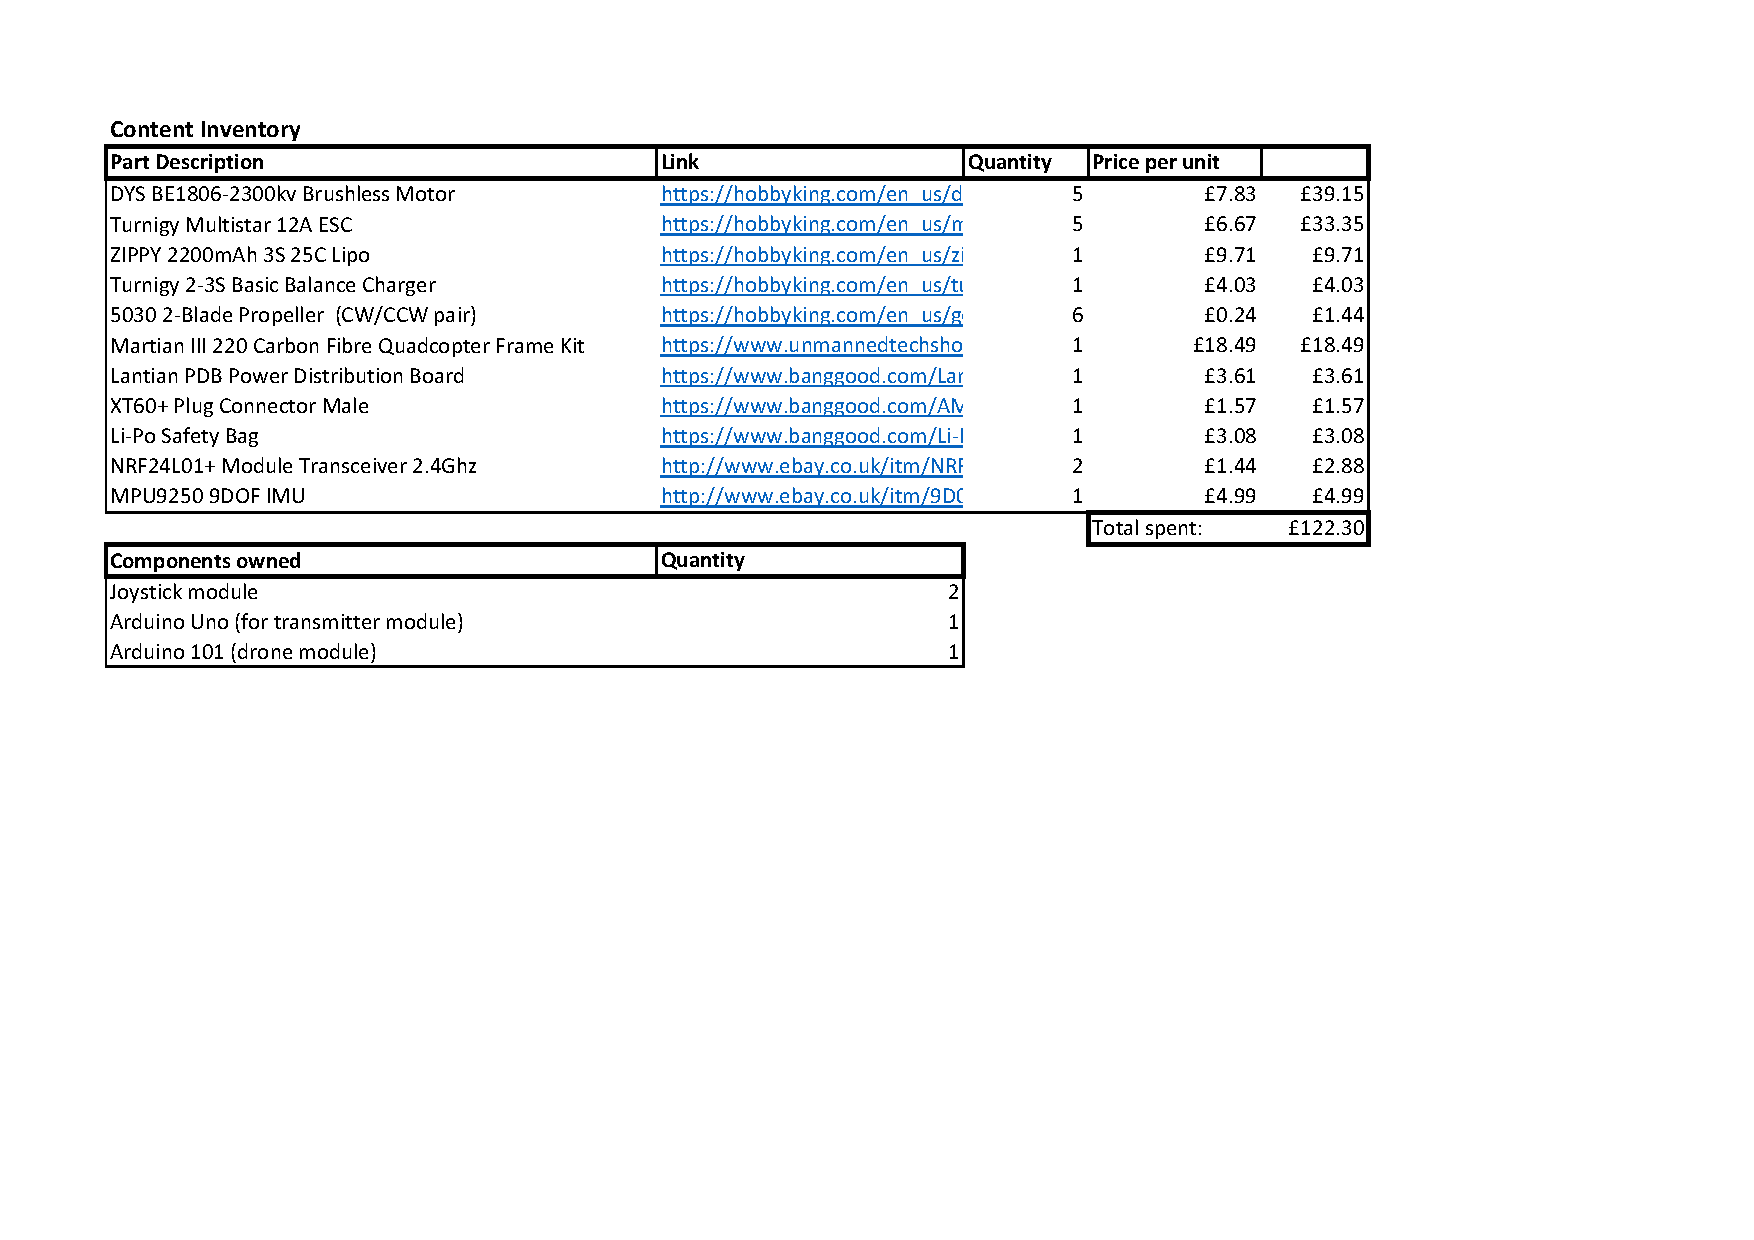
\includepdf[pages={1}, angle=-90, offset=1in -1in]{inventory.pdf}
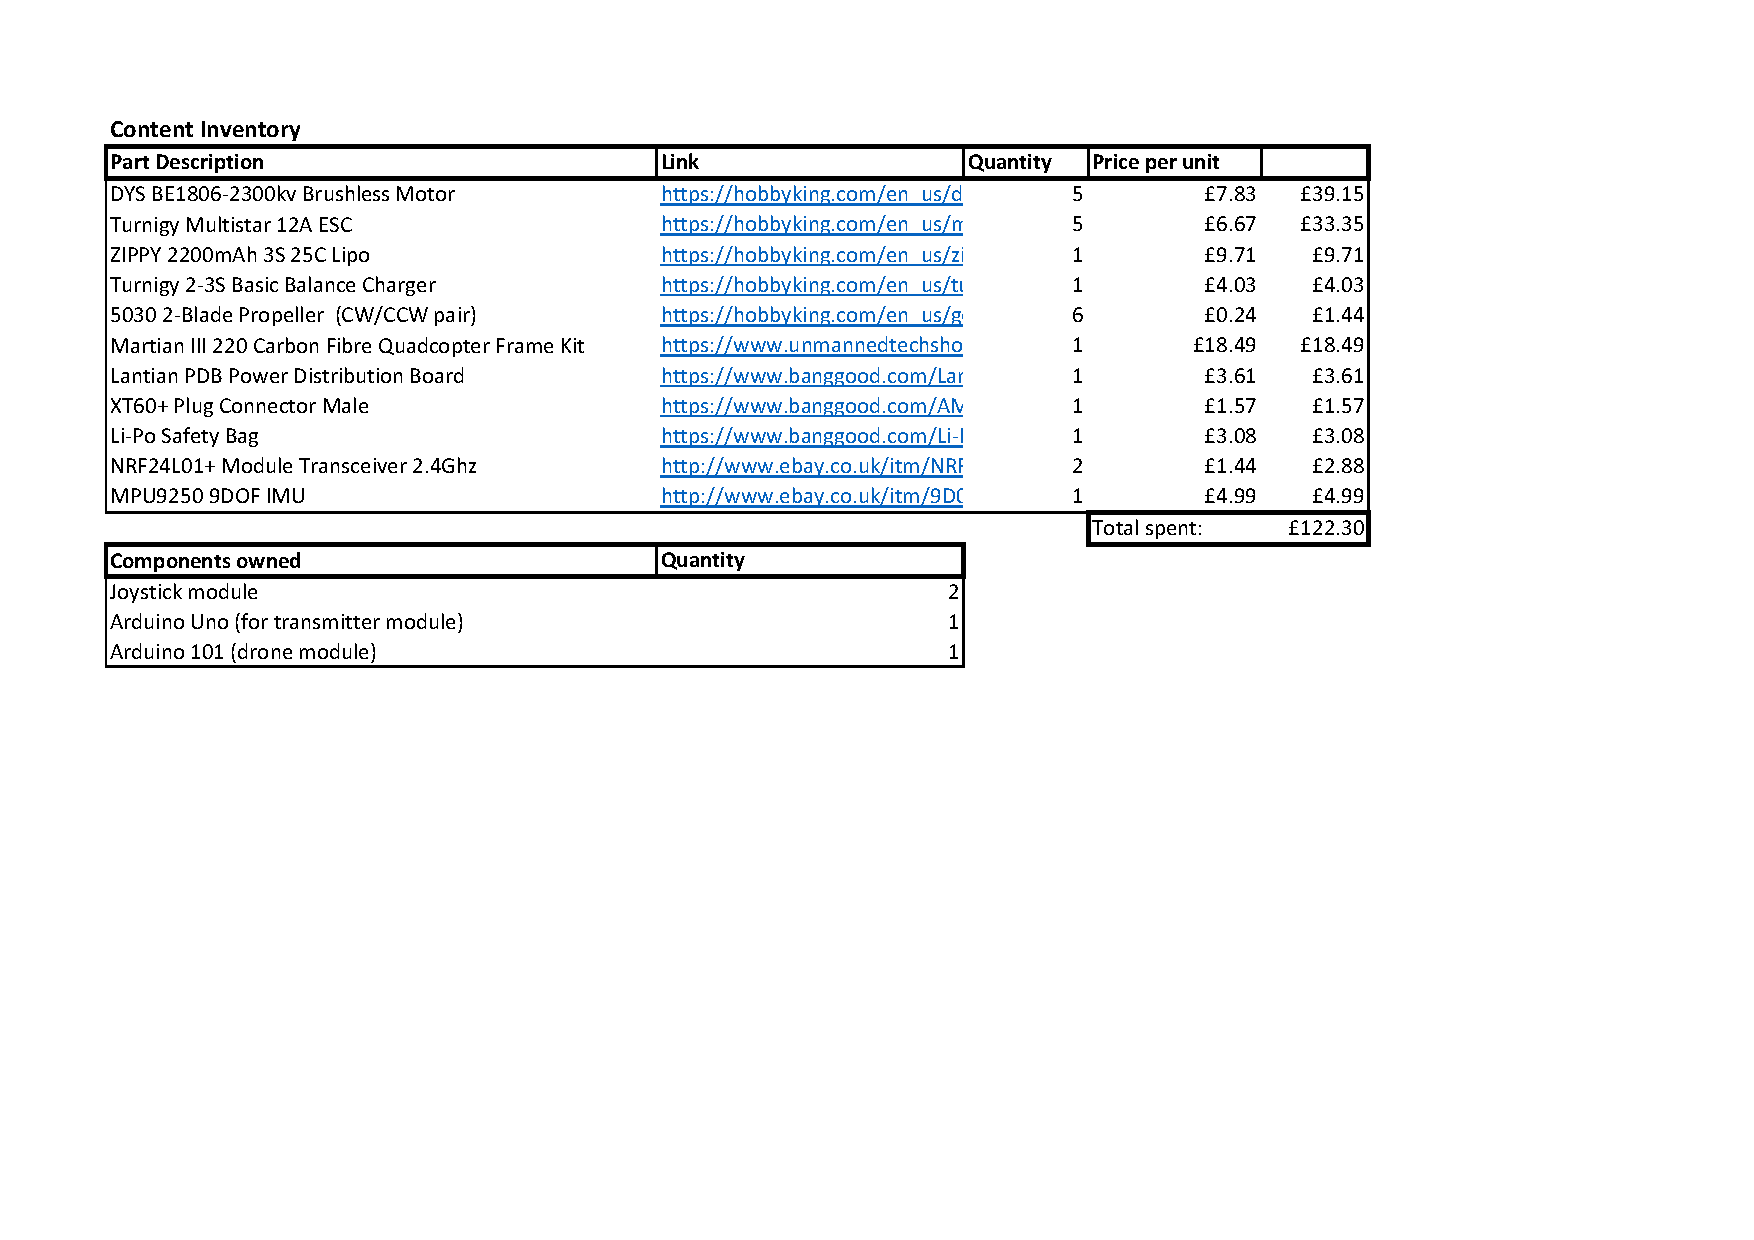
\includepdf[pages={1},pagecommand={\thispagestyle{plain}\invisiblesection{Inventory Content}}, angle=-90, offset=-1in -1in]{inventory.pdf} \label{Contents Inventory}

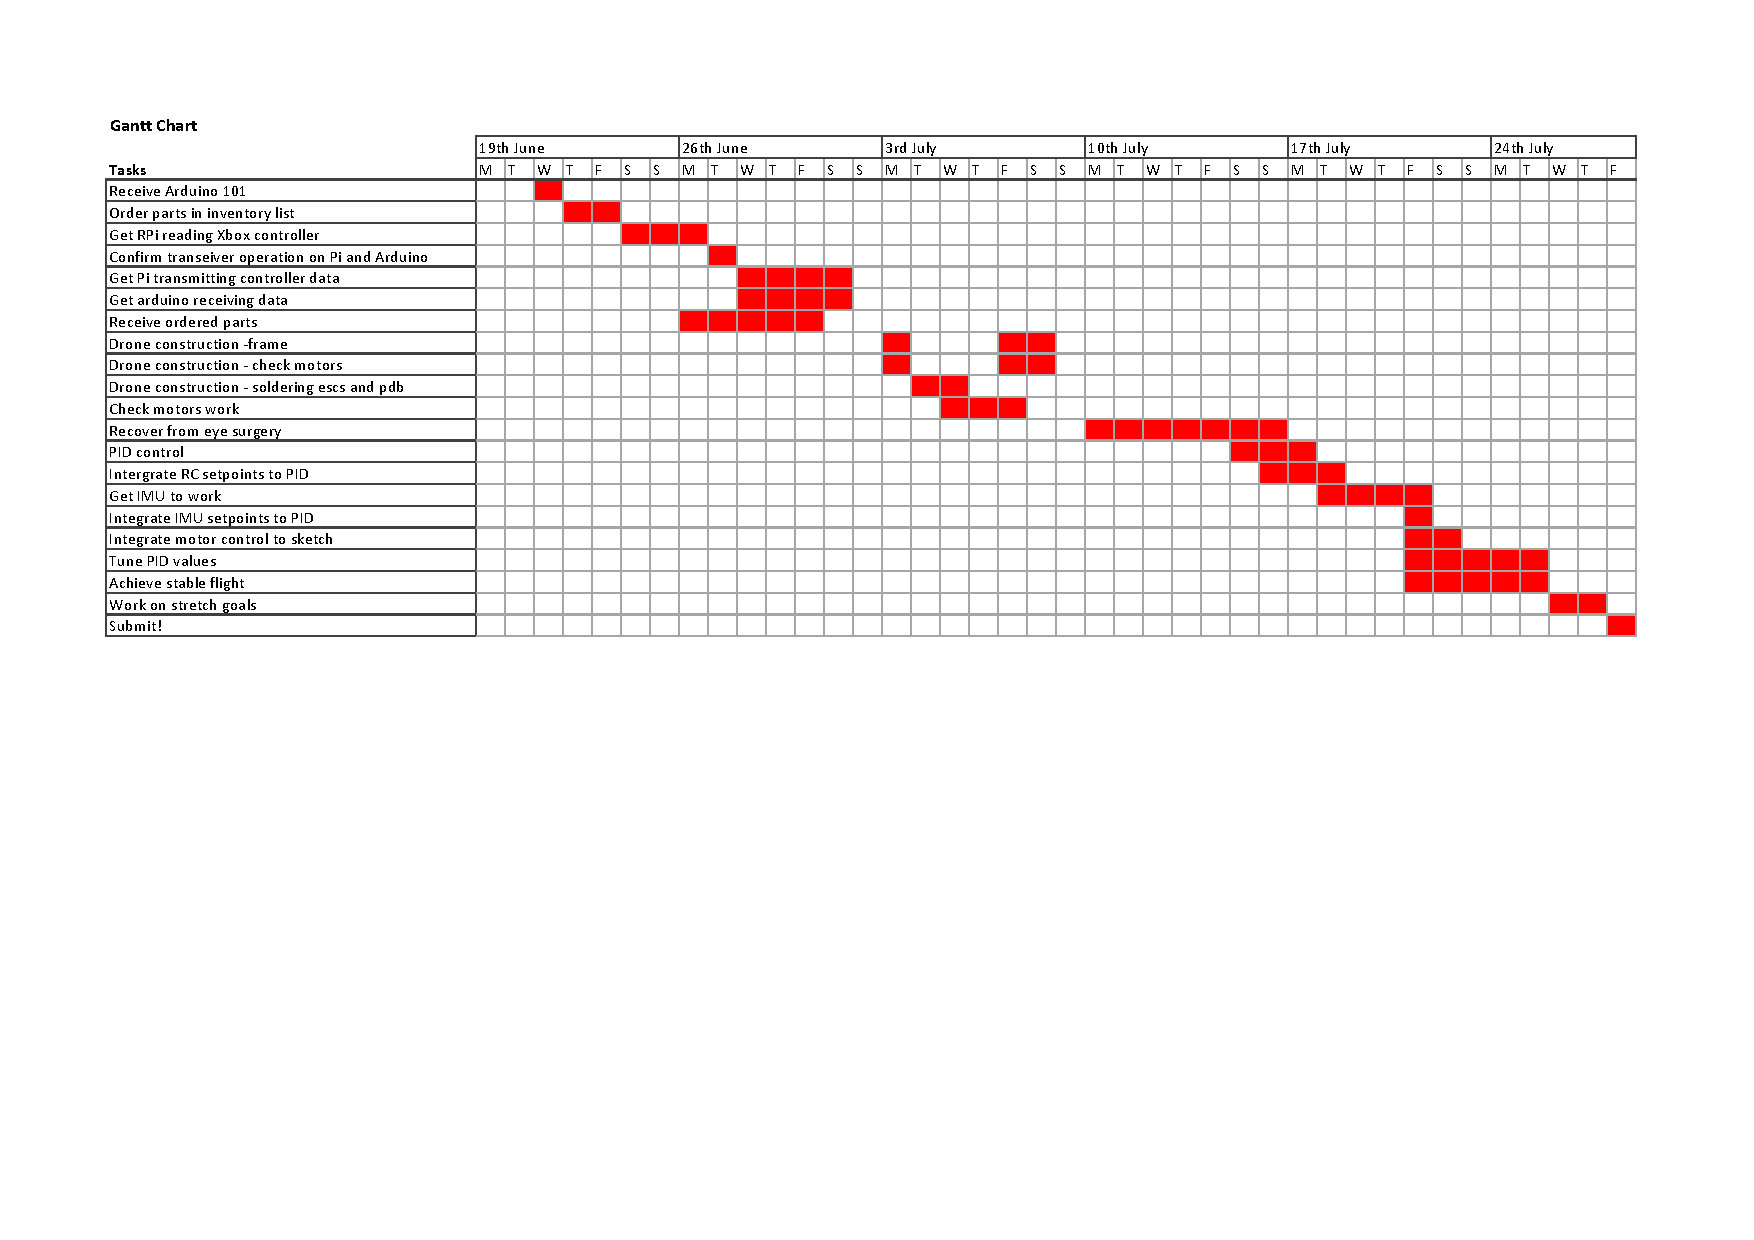
\includepdf[pages={1}, angle=-90, offset=1in -1in, pagecommand={\thispagestyle{plain}\invisiblesection{Gantt Chart}}]{Chart.pdf}
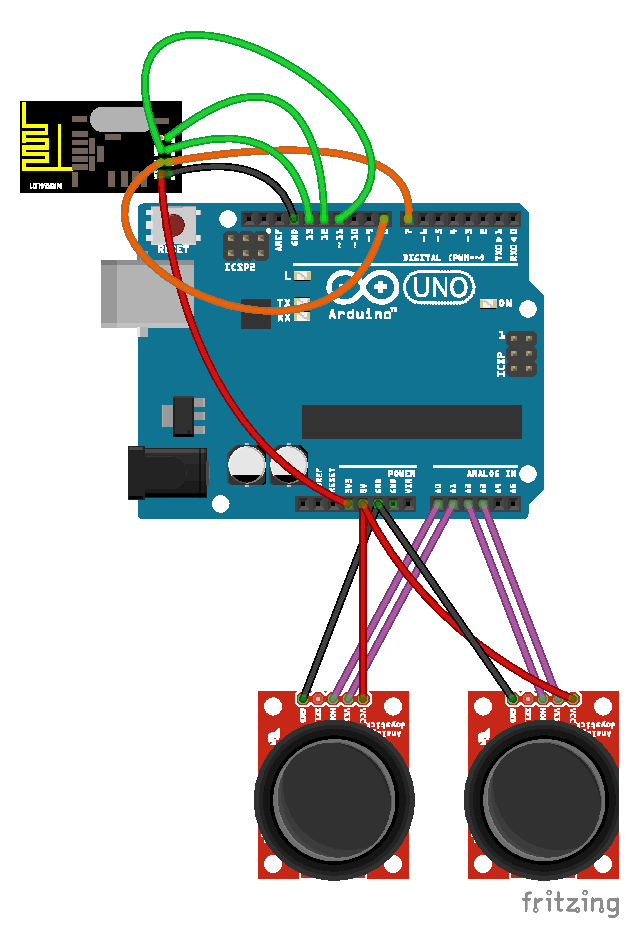
\includepdf[pages={1}, offset=-1in -1in, pagecommand={\thispagestyle{plain}\invisiblesection{Transmitter Wiring Diagram}}]{TRANSMITTERcurves_bb.pdf}
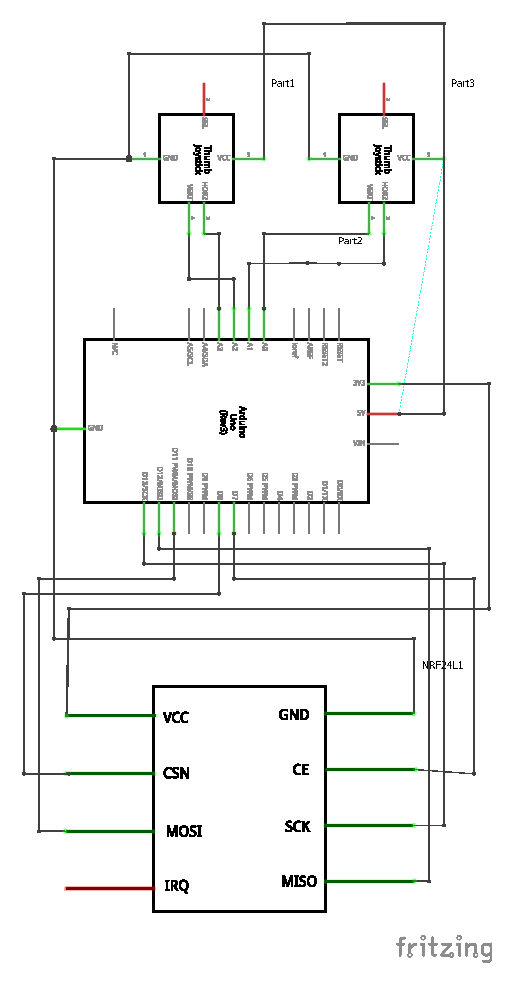
\includepdf[pages={1}, offset=1in -1in, pagecommand={\thispagestyle{plain}\invisiblesection{Transmitter Schematics}}]{TRANSMITTER_schem.pdf}
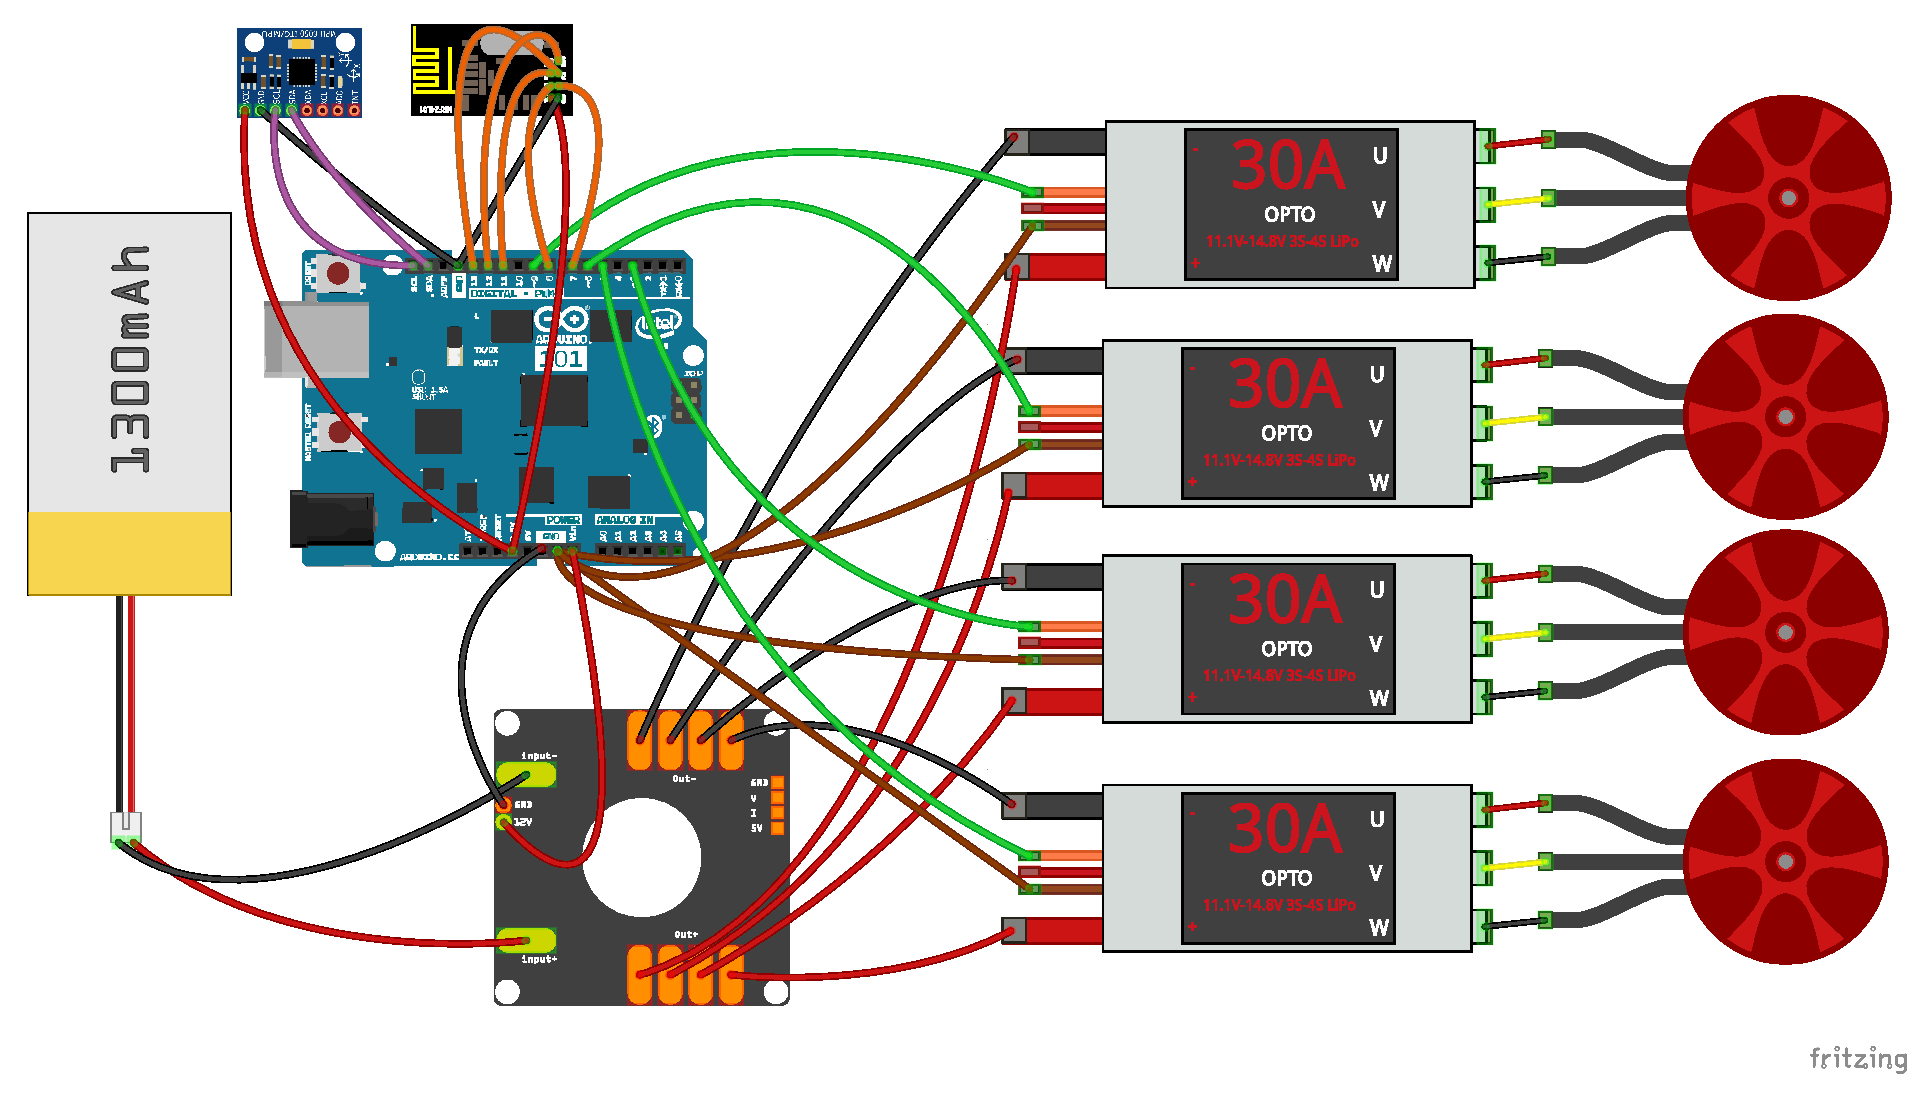
\includepdf[pages={1}, angle=-90, offset=-1in -1in, pagecommand={\thispagestyle{plain}\invisiblesection{Quadcopter Wiring Diagram}}]{drone_bb.pdf}
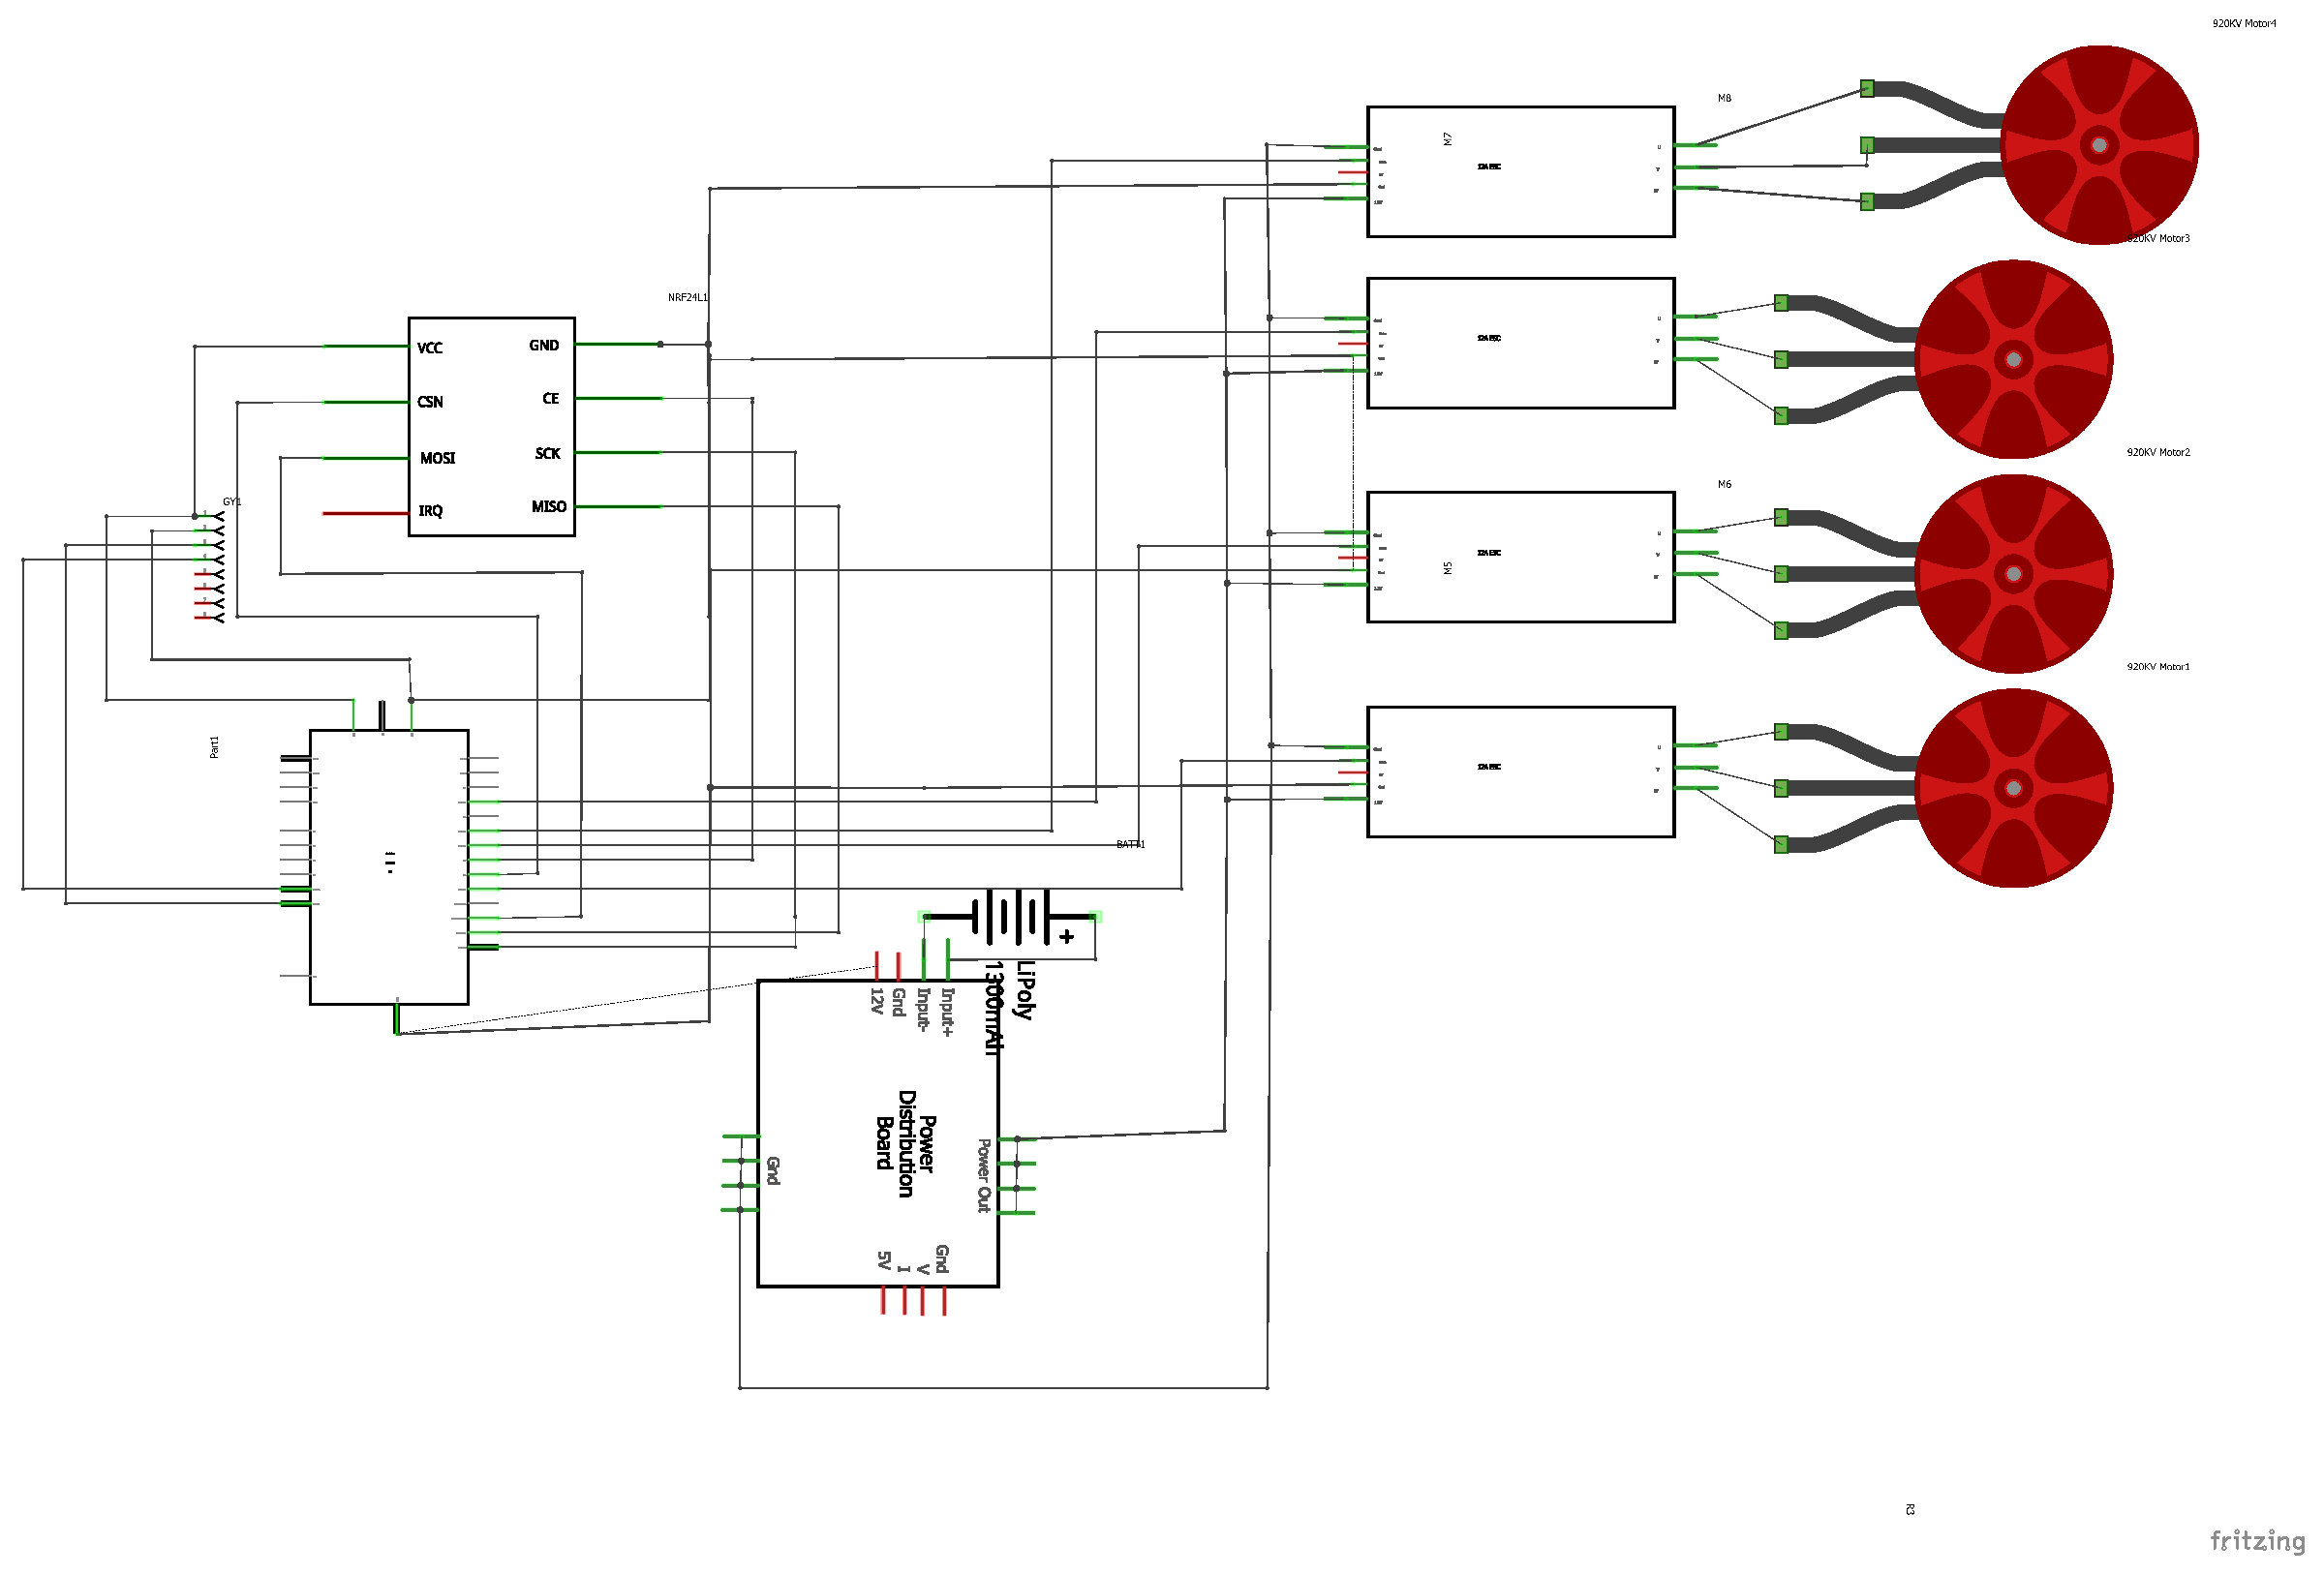
\includepdf[pages={1}, angle=-90, offset=1in -1in, pagecommand={\thispagestyle{plain}\invisiblesection{Quadcopter Schematics}}]{drone_schem.pdf}

\invisiblesection{Conclusion}\thispagestyle{plain}
\textbf{Conclusion}\\

There have been a number of changes made since my initial proposal; foremost the level of complexity of my drone. In just six weeks since receiving the Arduino 101, I’ve managed to design, build, program, and fly my very own drone. \\
Some of my initial plans were changed along the way. For example, my decision to use a Raspberry Pi connected to an Xbox controller was eventually scrapped in favour of making my own remote control transmitter with some joystick modules, buttons, and an Arduino Uno. I’ve also faced many mechanical issues whilst constructing the drone, resulting in solutions like cutting my own acrylic base plate to attach the Arduino to, and making my own standoffs to house the battery. And of course, what project would be complete without spontaneous hardware failures a week before submission? Fortunately speedy delivery times meant I was able to replace the failed ESC, and get the drone back in the air with a just hours to spare.
At the moment I have a drone that exhibits stable flight. I fully intend on continuing this project, and adding all the cool features I’d planned (what kind of drone doesn’t need a nerf gun?!). The beauty of using the Arduino 101 as a flight controller is the potential to grow and adapt the project in any direction I want to take it. \\
Finally, I would just like to thank everyone involved at Devpost and Intel for giving me the opportunity to do this! I’ve not only expanded my skills as a programmer, but also how to manage my time during a long project – something that will definitely come in useful for my University Electronics 3rd Year project in September!






	
\end{document}
%% ----------------------------------------------------------------
